\documentclass[12pt]{report}
\usepackage[english]{babel}
\usepackage{natbib}
\usepackage{url}
\usepackage[utf8x]{inputenc}
\usepackage{amsmath}
\usepackage{graphicx}
\graphicspath{{images/}}
\usepackage{parskip}
\usepackage{fancyhdr}
\usepackage{vmargin}
\usepackage{colortbl}
\usepackage{hyperref}
\setmarginsrb{3 cm}{2.5 cm}{3 cm}{2.5 cm}{1 cm}{1.5 cm}{1 cm}{1.5 cm}

\author{SOW Sokhna Maimouna} % Author

\makeatletter
\let\theauthor\@author
\renewcommand{\thesection}{\@arabic\c@section}


\makeatother

\pagestyle{fancy}
\fancyhf{}
\lhead{\theauthor}
\rhead{\rightmark}
\lfoot{Universite Paris Nanterre}
%\rfoot{Cosmo Consult}
\cfoot{\thepage}
\renewcommand{\footrulewidth}{0.4pt}%trait horizontal pour le pied de page

%*********************page de  fond **************************
\usepackage{eso-pic}
\newcommand\BackgroundPic{%
\put(0,0){%
\parbox[b][\paperheight]{\paperwidth}{%
\vfill
\centering
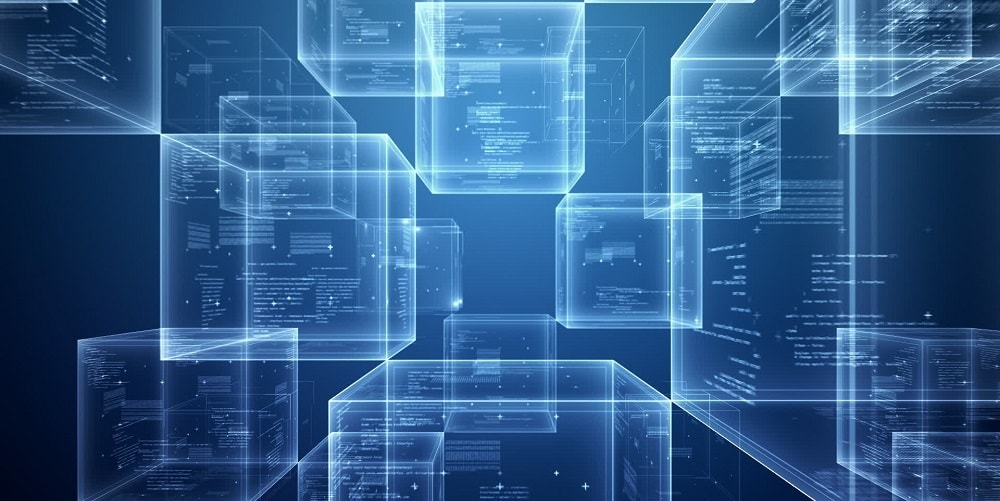
\includegraphics[width= 3\paperwidth,height=\paperheight,%
keepaspectratio]{couverture_blockchain_2}%
\vfill
}}}

\begin{document}
\AddToShipoutPicture*{\BackgroundPic}

%%%%%%%%%%%%%%%%%%
%%% First page %%%
%%%%%%%%%%%%%%%%%%

\begin{titlepage}
\begin{center}

%
\includegraphics[width=0.6\textwidth]{fac}\\[1cm]

{\large \textcolor{white}{\textbf{Méthodes Informatiques Appliquées à la Gestion des Entreprises}}}\\[0.8cm]


{\large \textbf{\textcolor{white}{Mémoire Master 2 Classique}}}\\[0.5cm]

\vfill

% Title
\textcolor{white}{\rule{\linewidth}{0.5mm} }\\[0.4cm]
{ \huge \bfseries \textcolor{white}{Comment intégrer les blockchains dans les transactions bancaires ?}  \\[0.4cm] }
\textcolor{white}{\rule{\linewidth}{0.5mm}} \\[1.5cm]

\vfill

% Author and supervisor
\noindent
\begin{minipage}{0.5\textwidth}
  \begin{flushleft} \large
    \emph{\textcolor{white}{Auteur :}}\\
   \textcolor{white}{Sokhna Maimouna \textsc {SOW}}\\
  \end{flushleft}
\end{minipage}%
\begin{minipage}{0.5\textwidth}
  \begin{flushright} \large
    \emph{\textcolor{white}{Encadrant :}} \\
   \textcolor{white}{Mme Marie-Pierre \textsc{Gervais}}\\
  \end{flushright}
\end{minipage}

\vfill

% Bottom of the page
{\large \textcolor{white}{Année scolaire \\ 2017 - 2018}}

\end{center}
\end{titlepage}

%page de garde
\thispagestyle{empty}
\newpage
~

\newpage
\section{Remerciements}
\hspace{1cm} MERCIIIIII.\\ 

\hspace{1cm} MERCIIIIII.\\ 


%%%%%%%%%%%%%%%%%%%%%%%%%%%%%%%%%%%%%%%%%%%%%%%%%%%%%%%%%%%%%%%%%%%%%%%%%%%%%%%%%%%%%%%%%
\newpage
\renewcommand{\contentsname}{Table des matières}
\tableofcontents
\pagebreak

%%%%%%%%%%%%%%%%%%%%%%%%%%%%%%%%%%%%%%%%%%%%%%%%%%%%%%%%%%%%%%%%%%%%%%%%%%%%%%%%%%%%%%%%%

\section{Introduction}
\hspace{1cm} Notre monde évolue au rythme des innovations et des nouvelles technologies. Aujourd'hui, nous sommes témoins d'une nouvelle révolution mondiale avec une portée assez difficile à mesurer mais mettant en avance des possibilités d'applications infinies. Cette révolution est marquée par le phénomène "\textbf{blockchain}". Elle est née du croisement d'une technologie cryptographique de pointe basée sur les registres distribués et d'un contexte sociologique opportun. Le cas de la blockchain est juste \textit{phénoménale}. En effet la rapidité de son développement technologique coïncide avec un contexte sociologique favorable, ce qui augmente les chances de tirer profit des grandes innovations technologiques en les transformant en un vrai usage. \\

\hspace{1cm} Derrière ce concept de blockchain se cachent les cryptomonnaies qui se \\démarquent des monnaies traditionnelles sur différents plans. Non seulement elles sont dématérialisées, anonymes, sécurisées mais ces devises peuvent s'échanger entre elles et permettent de faire des transactions bancaires. Et pendant ce temps, nous avons un système bancaire avec un réseau trop organisé, encadré et centralisé qui est bien construit et trop hiérarchisé avec des dirigeants qui contrôlent tout le système et ont toujours le dernier mot.\\

\hspace{1cm} Face à cette situation, il me semble opportun de s'interroger sur la performance et l'avenir des banques. Puisque c'est assez difficile de contourner les banques, cela me pousse à chercher comment procéder à mettre en place en place les blockchains afin de faciliter le monde monétaire de demain? Comment intégrer les blockchains dans les transactions bancaires ? Quels sont les acteurs à impliquer ? Tellement de questions qui me motivent à faire à faire une étude approfondie et dans la mesure du possible trouver une solution pour faire cohabiter les banques et les blockchains.\\

\hspace{1cm} A travers ces lignes je vais d'abord expliquer ce que c'est la blockchain en partant de sa création jusqu'à son processus final en détaillant son architecture et voir les différentes blockchains qui existent de nos jours. Ensuite j'étudierais l'impact des blockchains dans l'actualité économique sans oublier de mettre en évidence les faiblesses de cette nouvelle technologique et répondre aux questions posées précédemment...... QUOI RAJOUTER OU COMMENT REFORMULER


%%%%%%%%%%%%%% Glossaire %%%%%%%%%%%%%%
\newpage
\section{Glossaire}
\begin{tabular}{|c|c|}
\hline 
\rowcolor{green}KEY & Value \\

\hline
Subprimes & Prêts immobiliers accordées aux américains ne remplissant \\ & pas les conditions pour un prêt classique \\ 

\hline 
BTC & Symbole utilisé pour représenter l'unité de compte du bitcoin \\

\hline
Cyber-marchand & Commerçant proposant ses services via un site de e-commerce \\

\hline
FEVAD & Fédération du e-commerce et de la vente à distance\\

\hline
TPE & Terminal de paiement électronique\\

\hline
Coin & Terme utilisé pour désigner les monnaies bitcoin\\

\hline
GBP & Code qui signifie : livre sterling, la monnaie du Royaume-Uni\\

\hline
USD & United States dollar, code de la monnaie des États-Unis \\

\hline
EUR & Code qui désigne : Euro, la monnaie européenne \\

\hline
QR & Acronyme de Quick Response et qui est un,code barre 2D\\

\hline
IBM & International Business Machines Corporation, est une société \\ & multinationale américaine\\

\hline
C2C & Consumer to Consumer, regroupe les activités entre consommateurs\\  

\hline
P2P & Peer-to-Peer, modèle de réseau où chaque client est aussi un serveur\\

\hline
B2B & Business to Business, entreprise qui vise une clientèle d'entreprises\\

\hline
B2C & Business to Consumer, entreprise qui vise une clientèle de consommateurs\\

\hline
UE & Union Européenne \\

\hline 
\end{tabular} 

\newpage
\section{Fonctionnement de la blockchain}

\hspace{1cm}  PHRASE OU PAS PHRASE

%%%%%%%%%%%%%% Historique %%%%%%%%%%%%%%

	\subsection{Historique}
\hspace{1cm} Tout a commencé par un groupe de 'geek' auto-organisé, sans hiérarchie et sans État qu'on appelle des \textbf{crypto-anarchistes}. Ces crypto-anarchistes savaient coder les données de façon à ce que personne d'autre que le destinataire ne puisse les déchiffrer. Ils se sont mis à "crypter des monnaies" d'où la naissance des\textbf{ monnaies virtuelles} appelées aussi \textbf{cryptomonnaie}. Si ces cryptomonnaies remontent aux années 70, ce phénomène devient célèbre qu'en début de 2009 avec la création de la blockchain et du bitcoin.\\

\hspace{1cm} En effet vers 2008, il y a eu une crise financière des subprimes. Les banques déclenchent alors la planche à billet afin de créer des euros et des dollars pour maintenir le système bancaire à flots. Et c'est vers cette même période précise qu'un certain \textbf{Satoshi Nakamoto}, un pseudo qui lui est attribué, publie un livre blanc de 10 pages, dans un forum de discussion, appelé \textbf{\textit{Bitcoin - A Per to Per Electonic Cash System }} qui va révolutionner le monde monétaire. Par la suite, plusieurs personnes ont prétendu être Nakamoto mais nous n'avons jamais pu découvrir le vrai cerveau qui se cachait derrière avec un fortune estimée à \textbf{980.000 token} soit \textbf{5.473.465.943 euros}. Il est resté actif jusqu'à mi 2010 pour ensuite disparaître des radars. C'est ainsi qu'on assiste à la naissance  de la première monnaie virtuelle décentralisée, qui fonctionne principalement avec la blockchain. \\ 

\hspace{1cm} De ce fait la première blockchain est apparue avec la monnaie numérique bitcoin. Aussitôt le marché virtuel se met à utiliser la technologie de la blockchain et plusieurs activités ont tourné autour de cette technologie naissante. Des plate-formes, des sites Internet et même des applications ont été mis en place pour la gestion des monnaies virtuelles et une utilisation permanente des blockchains.


%%%%%%%%%%%%%% Archi %%%%%%%%%%%%%%

\newpage
	\subsection{Architecture de la blockchain}

\hspace{1cm} Qu'est que la blockchain? Certains diront que c'est juste une écriture comptables d'opérations numériques qui sont partagées entre de multiples parties prenantes. D'autres diront c'est un ensemble de réseau maillé d'ordinateurs reliés entre eux. Tellement de définitions lui sont attribuées. Mais quand est-il réellement de ce nouveau fléau? Comment est elle structurée? Quelles sont ses composantes? Essayons plutôt d'expliquer le mécanisme de la blockchain pour en sortir une définition adéquate.

\hspace{1cm} Prenons un livre où nous allons écrire toutes les dépenses que chacun a réalisé avec les montants et les dates.

\begin{itemize}
    \item Le 01/08/2009 à 16h : Alice paie 250 euros à Bob 
    \item Le 03/08/2009 à 20h : Bob paie 30 euros à Carole
    \item Le 03/08/2009 à 22h : Alice paie 15 euros  à Carole
    \item Le 04/08/2009 à 19h : Carole paie 20 euros  à Clara
    \item etc.
\end{itemize}

\begin{center}
    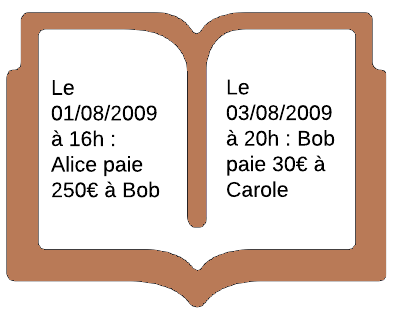
\includegraphics[width=0.5\textwidth]{livre_compte}

    \textbf{\underline{Livre de compte}} \\[1cm]
\end{center}

Nous avons ici un grand livre qui dit qui a payé qui. Il n'est dit nulle part de combien d'argent vous disposez, mais nous le savons bien car nous avons toutes les échanges, leurs détails et le contenu du compte initial, donc il suffit juste de faire ses déductions. Par contre nous pouvons avoir des centaines d'échanges alors que le nombre de ligne d'un livre est limité. Comment faire dans ce genre de cas alors? C'est très simple il faut prendre un nouveau livre et continuer à remplir. Et pour ne pas se perdre les livres sont numérotés. Chaque livre contient le résumé du précédent, ce qui permet de les relier entre eux et d'avoir une continuité. Nous obtenons ainsi un enchaînement de livres remplis de toutes les échanges.\\

\begin{center}
    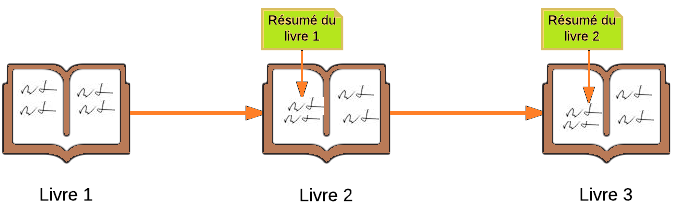
\includegraphics[width=1\textwidth]{livre_compte_2}

    \textbf{\underline{Enchaînement des livres}} \\[1cm]
\end{center}

\hspace{1cm} Et dans le monde de la cryptomonnaie, à la place de ces livres, nous avons des fichiers appelés \textbf{blocs}. Ces blocs sont construits les uns à la suite des autres, formant ainsi une \textbf{chaîne de blocs}. D'où le nom de \textbf{Blockchain}.\\

\hspace{1cm} Mais comment est ce possible de résumer les informations du bloc précédent dans le bloc suivant? Ils utilisent ce qu'on appelle les \textbf{Hash} qui sont des fonctions mathématiques permettant de transformer n'importe quelles données en entrée en un grand nombre hexadécimal composé de lettres et de chiffres en sortie. Ces fonctions nous permettent non seulement de relier nos blocs mais aussi d'avoir la garantie que le contenu du bloc n'a pas été changé. En effet les fonctions de hashage ne marchent que dans un seul sens, ce qui assure la sécurité des blockchains. Si vous modifiez l'historique, cela ne correspondrait plus avec le hash du 1er bloc qui est dans le 2ème bloc et ainsi de suite.\\

\hspace{1cm} Ainsi ce sont les transactions effectuées entre les utilisateurs du réseau qui sont regroupées en blocs. Chaque bloc sera validé par les noeuds du réseau, on les appelle les \textbf{mineurs},  en fonction des techniques qui dépendent du type de blockchain. Dans la blockchain du bitcoin, la cryptomonnaie la plus populaire, cette technique s'appelle le \textbf{Proof-of-Work}, ce qui signifie \textbf{preuve de travail}. Elle consiste en la résolution de problèmes algorithmiques. Et dès que le bloc est validé, il est horodaté et est ajouté à la chaîne de blocs, ce qui implique que la transaction est visible aussi bien pour le récepteur que pour l'ensemble du réseau.

\begin{center}
    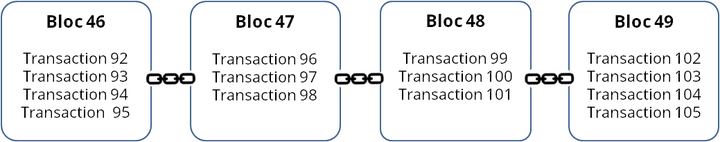
\includegraphics[width=1\textwidth]{block_schema}

    \textbf{\underline{Les transactions dans une blockchain}} \\[1cm]
\end{center}

\hspace{1cm} Ce concept de \textbf{minage} fait qu'il n'existe pas de banque centrale qui produit ou gère les monnaies. En effet ce sont les ordinateurs  appartenant au même réseau qui font tous le travail. Ce qui fait que tout est sécurisé par le procédé cryptographique. Et c'est la difficulté pour quiconque de résoudre les preuves de calcul qui assure la sécurité de toutes les transactions.\\

\hspace{1cm} Ainsi je définirais plutôt la blockchain comme une technologie de transmission d'informations et de stockage. Elle a une base de données très sécurisée et dont la gestion est traitée par un ensemble de réseau d'ordinateurs connectés entre eux et qui stockent ces données de manière distribuée. Cette base contient toute l'historique de toutes les transactions entre les utilisateurs depuis sa création et est en même temps partagée sans intermédiaire. Ce qui donne la possibilité à chaque utilisateur de vérifier la validité de la chaîne.

%%%%%%%%%%%%%% Types de blockchain %%%%%%%%%%%%%%

	\subsection{Les types de blockchain}
\hspace{1cm} Nous avons différents types de blockchain en fonction des secteurs. 

\begin{enumerate}

    \item \underline{\textbf{Blockchain publique}}\\ [0.3cm]
La blockchain publique est caractérisée par le fait que tous les noeuds du réseau d'échange sont contrôlés par le fameux réseau peer-peer. Pour y accéder, il y a aucune permission à demander et aucune barrière d'entrée. N'importe qui peut faire une transaction ce qui veut dire que tous les acteurs sont égaux dans leur participation du réseau. C'est le cas des monnaies virtuelles \textbf{bitcoin} et \textbf{ethereum} pour lesquels chacun a libre accès au registre et participe au même titre au processus d'approbation, celui qui permet de décider lequel des blocs doit être ajouté ou pas à la chaîne et qui définit l'état actuel du système.\\ 

\newpage
    \item \underline{\textbf{Blockchain privée}}\\[0.3cm]
la blockchain privée a son propre réseau privé dont l'accès est strictement confié au gérant qui, lui seul peut faire des modification dessus. Donc personne ne peut y accès sans y être autorisé. Cette blockchain est beaucoup utilisée par les banques grâce à sa gouvernance simplifiée, ses coûts réduits, sa rapidité, sa confidentialité surtout et du fait que les acteurs sont connus. Par contre cette blockchain perd tout son charme du moment qu'elle est privée. En effet comme l'a si bien dit \textbf{Juge David Teruzzi}, expert en bitcoin, je cite "Cette blockchain n'est pas très intéressante. Elle est certe scalable à l'infini, contrairement à la blockchain publique, mais son intérêt est limité puisqu'elle ne fait pas le lien entre différents acteurs". 

    \item \underline{\textbf{Blockchain hybride}}\\[0.3cm]
Nous avon aussi les blockchains hybrides. Vous avez les droits d'écritures et de  modifications et certains noeuds peuvent êtres rendus publics et d'autres privés.C'est le cas du \textbf{consortium} qui est une blockchain regroupant plusieurs acteurs mais n'est ni publique ni ouverte à tout le monde. Les acteurs ont certains droits d'accès mais les décisions sur la blockchain sont prises par la majorité d'entre eux. Cette blockchain est plutôt adaptée aux contextes régulés et est utilisée à l'international comme IBM.\\

\end{enumerate}

\hspace{1cm} Tous ces types de blockchains, publiques, privées et consortium, pourraient finir par cohabiter. Chacune est spécialisée sur des applications adéquates. Et comme le dit  \textbf{Luca Comparini}, un blockchain leader chez IBM France, je cite"La blockchain publique est idéale pour les marchés C2C et P2P, tandis que les blockchains privées et les consortiums sont davantage adaptés au B2B. Pour le B2C, cela dépendra des contraintes du secteur".  Ce qui pousse aux mineurs de prévoir des passerelles entre les différentes blockchains afin d'assurer leur une possibilité de communication entre les systèmes.\\


%%%%%%%%%%%%%% Système actuel %%%%%%%%%%%%%%
\newpage
\section{Système des transactions bancaires}

\hspace{1cm} Avant la mise en place des premières cartes de paiement, la plupart de la population gardait leurs fonds sur eux ou à leur domicile. Ce qui veut dire que ces sommes pouvaient être dérobées et quand ça arrivait ils n'étaient pas remboursés. Donc faire des achats n'était pas sans risque pour l'intégrité de l'acteur et de ses économies. De plus il fallait avoir la totalité de la somme du montant au moment d'un achat pour effectuer l'opération, ce qui rendait les transactions un peu compliquées. Il était aussi facile de faire des erreurs de calculs dès que la monnaie était échangée et les transactions bancaires n'était pas répertoriée directement.\\

\hspace{1cm} Pour faciliter les transactions bancaires, ils ont mis en place un système appelé la \textbf{monétique} qui regroupe l'ensemble des processus nécessaires à la création d'une carte, la lecture des informations associées et la gestion des transactions monétaires. Ces transactions monétaires ont toutes des processus différents et spécifique. Nous allons prendre comme exemple le processus d'une transaction par carte bancaire qui est très courant.Il met en jeux plusieurs acteurs tels que : 

\begin{itemize}
    \item Un \textbf{émetteur}, qui peut être la banque du client
    \item Un \textbf{porteur} de carte, c'est à dire le client
    \item Un \textbf{accepteur} du moyen de paiement qui est très souvent le commerçant
    \item Un \textbf{acquéreur} de données de transaction dont la banque émettrice
\end{itemize}

Ces principaux acteurs communiquent indirectement mais de façon coordonnée et sécurisée.En effet: 

\begin{itemize}
    \item il y a d'abord le client qui crée son compte dans une banque. La banque lui envoie une carte associée au compte et qui lui permettra de faire tous les achats par la suite.
    \item Dès lors le client est libre de faires ses transactions chez un commerçant. Parfois il peut y avoir des demandes d'autorisation afin de vérifier la solvabilité du compte ainsi que la validité de la carte.
    \item Après la transaction le commerçant obtient un TPE qui va lire la carte et transmettre les données de la transaction. Cette étape est appelée la \textbf{télécollecte}. 
    \item Une fois cette télécollecte effectuée, la banque du client et celle du commerçant communiquent entre elles afin d'effectuer ce qu'on appelle la \textbf{télécompensation} qui va permettre de débiter le compte du client et créditer celui du commerçant. \\[1cm]
\end{itemize}

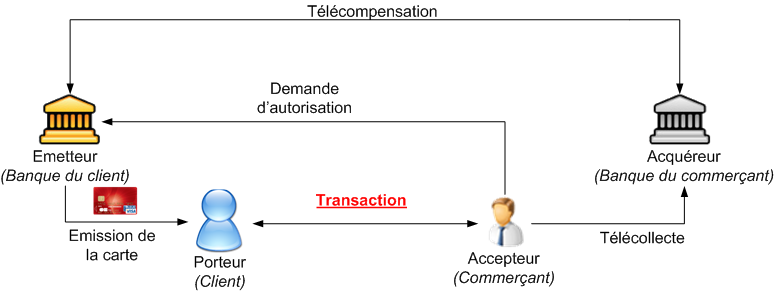
\includegraphics[width=1\textwidth]{process_transaction}
\begin{center}
   \textbf{\underline{Processus d'une transaction bancaire}} \\[1cm]
\end{center}

\textbf{TROUVER UNE PHRASE POUR INTRODUIRE LES TRANSACTION}
\hspace{1cm} Ce système monétique ...... 

%%%%%%%%%%%%%% Carte bancaire %%%%%%%%%%%%%%
    \subsection{Les transactions par carte bancaire physique}
\hspace{1cm} La carte bancaire est le moyen de paiement le plus utilisé en France. Elle représente presque \textbf{50\%} des paiements en 2014 avec \textbf{9,49 milliards} de paiements effectués par cartes. Cette carte est d'une utilisation simple que ce soit pour un paiement ou pour un retrait et est acceptée presque par tous les commerçants. \\ A CONTINUER.....

\hspace{1cm} Cependant la carte nous impose un coût annuel assez élevé en fonction des banques ainsi que des frais sur certains retraits et paiements avec des assurances sur les achats effectués. De même il exige très souvent un montant minimum d'utilisation chez les commerçants. Ils ont mis en place des plafonnements de dépenses par mois ou par semaine en fonction des banques, ce qui est très embarrassant à cause du manque de flexibilité. Avec cette carte vous n'avez pas non plus la possibilité de faire des paiements entre particuliers. Et utiliser sa carte à l'étranger équivaut à payer des frais exorbitants.

%%%%%%%%%%%%%% E-commerce %%%%%%%%%%%%%%
    \subsection{Le monde du E-commerce}
\hspace{1cm} Le e-commerce est l'ensemble des transactions commerciales s'opérant à distance via des interfaces électroniques et digitales. Aujourd'hui c'est un secteur en pleine expansion. Les achats et ventes se passent le plus souvent par le biais du numérique au détriment des marchés physiques traditionnels. L'e-commerce prend de plus en plus d'ampleur. en effet, une étude de la Fevad montre un chiffre d'affaire qui s'élève à \textbf{72 milliards d'euro} en 2016 pour un total de plus de \textbf{200 000 sites marchands}. Nous avons environ \textbf{2000 euro par année} dépensé par un e-acheteur pour \textbf{28 transactions}. En 2016 l'e-commerce représentait \textbf{8\%} du commerce de détail.\\

\hspace{1cm} Par contre ces e-commerçants investissent beaucoup sur des plate-formes qui jouent le rôle d'intermédiaire entre eux et les acheteurs. Ce qui les pousse parfois à augmenter le prix de leurs marchandises pour en tirer bénéfice.\\ De même pour un paiement en ligne certains sites vous demanderont vos données personnelles, quelque chose dont vous ne connaissez où ça peut vous amener. Le manque de confiance dans les moyens de paiements sur les sites d'e-commerce et la peur de se faire arnaquer pose un vrai problème au grand public et porte préjudice aux e-commerçants. 


%%%%%%%%%%%%%% Transaction papier %%%%%%%%%%%%%%
    \subsection{Les transactions sur papier}
\hspace{1cm} Nous faisons différentes transactions basées principalement sur les documents telles que:

\begin{itemize}
    
    \item \textbf{Billet à ordre}: C'est un écrit par lequel le client s'engage à payer une certaine somme avec une échéance déterminée à son fournisseur.
    
    \item \textbf{Chèque}: C'est un écrit par lequel une personne donne l'ordre de payer une certaine somme, prélevable immédiatement sur les fonds portés au crédit de sont compte, à lui même ou à un tiers.
    
    \item \textbf{Lettre de change }: C'est un écrit par lequel un créancier d'origine donne à un débiteur l'ordre de payer avant l'échéance fixée, une certaine somme à une troisième personne appelée qui est le bénéficiaire.
    
    \item \textbf{Traite} : C'est un titre qu'on peut négocier et qui présente, au profit du porteur, une créance d'une certaine somme et sert à son paiement. Il doit suivre un formalisme très rigoureux pour sa validité et son efficacité. Contrairement au chèque, il n'est pas encaissable immédiatement et ils sont beaucoup plus utilisés que les billets à ordre.

\end{itemize}
    
\hspace{1cm} Ces moyens de transaction bancaires sont quotidiennement utilisés en France, particulièrement les chèques, grâce à leur gratuité d'acquisition. Avec une transaction par "papier", vous avez la possibilité de garder une trace du paiement.  De plus les paiements sont gratuits ainsi que leurs acquisitions.\\

\hspace{1cm} Mais il se trouve que certains commerçants n'acceptent pas les chèques à partir de certains montant, par mesure de sécurité et à cause  des nombreux chèque impayés. Effectivement vous n'avez aucune garantie que les chèques encaissés ne sont pas sans provisions. En plus de tout ça il y a beaucoup de fraudes sur les chèques aujourd'hui \\


%%%%%%%%%%%%%% transfert d'argent %%%%%%%%%%%%%%
    \subsection{Les transferts d'argent}
    
Il existe plusieurs types de transferts  d'argent. Parmi eux nous pouvons en citer: 

\begin{enumerate}
    \item Virement bancaire: Ça consiste à envoyer ou recevoir de l'argent par le biais d'un compte bancaire. Vous avez la possibilité de faire des virements: 
    
    \begin{enumerate}
        \item ouverts dans la même banque, ce qu'on appelle \textbf{virement interne}
        \item ouverts dans deux banques différentes, appelé \textbf{virement externe}
        \item réalisés dans le même pays, appelé \textbf{virement domestique}
        \item réalisés entre deux pays de l'UE. Ce virement doit êre inférieur à \textbf{50 000 euros}
        \item réalisés hors UE, à l'étranger
        \item réalisés ponctuellement ou permanents 
    \end{enumerate}
Les virements bancaires sont des moyens de paiement à distance particulièrement utiles surtout s'il s'agit de grosses sommes ou de paiement de dépenses contraintes. Vous avez une traçabilité bien détaillée.\\

\hspace{1cm} Ce moyen de paiement est sûr mais n'est pas souvent gratuit. En effet chaque banque applique son propre tarif. Et si c'est un virement dans une autre monnaie, devise, il y a un taux d'échange qui est appliqué. Ce coût dépend aussi des devises et peut vous coûter très cher. Un autre problème est lié au délai de transaction. Pour un virement dans l'UE, un virement peut durer maximum 4jours, mais en dehors de l'UE il n'existe pas de délai maximum ce qui fait qu'un virement peut durer assez longtemps. Et même pour certaines banques,  le virement à l'intérieur de la France peut s'avérer long, et nécessite parfois une autorisation préalable de la banque et l'enregistrement du compte ce qui peut prendre plusieurs jours. De même les virements permanents sont débités automatiquement, ce qui oblige à avoir la somme due, sinon des frais peuvent s'appliquer.

    \item Transfert d'espèce: Nous pouvons en citer quelques uns : 
    
    \begin{enumerate}
        \item Mandat cash
        \item Western Union
        \item MoneyGram 
    \end{enumerate}
    
Les transferts d'argent par mandat ou western sont particulièrement destinés aux personnes ne détenant pas de compte bancaire. Ces transactions peuvent vous permettre d'envoyer de l'argent à une personne n'ayant pas de carte d'identité, mais avec maximum 400 euros.\\

\hspace{1cm} Ces transferts sont rapides et efficaces, mais est très coûteux surtout à l'international.D'après les données de la Banque Mondiale en 2015,  presque \textbf{10\%} de commissions sont prélevés par les plateformes d’échange dans certaines régions. la diaspora africaine dépense ainsi \textbf{2 milliards d'euros} par an à cause des coûts d'envoi des transferts d'argent.  Ces frais de transfert dont les coûts s'élèvent à \textbf{12\%}, soit le double de la moyenne mondiale. Il y a aussi les coûts changent souvent à cause des fluctuations de devise\\

\hspace{1cm} En plus de ces frais, viennent se rajouter les restrictions. En effet certains opérateurs de transfert peuvent interdire des transactions commerciales, c'est à dire une transaction liant un fournisseur à un commerçant. Ils vous obligent ainsi à faire des transactions uniquement liées aux remboursements, aux dons et aux familles.\\
    
\end{enumerate}

%%%%%%%%%%%%%% Pret bancaire %%%%%%%%%%%%%%
    \subsection{Prêts bancaires}
    
\hspace{1cm} Faire un prêt consiste à remettre des fonds à un bénéficiaire, moyennant le plus souvent à un intérêt à verser au prêteur. Donc il y a un engagement de remboursement à respecter. Ces prêts sont profitables pour un financement à un projet et utiles pour tous ceux qui ont un besoin urgent. Mais 
le problèmes avec ces prêts c'est qu'ils vous proposent un taux d'intérêts élevés, augmentant ainsi le taux d'endettement. Ces prêts sont d'utilité mais à quel prix? Est ce qu'avec ce système ça vaut le coût ?

%%%%%%%%%%%%%% Conclusion de ce chapitre %%%%%%%%%%%%%%
\hspace{1cm} Toutes ces transactions transactions sont indispensables à notre quotidien. Mais il se trouve que nous avons des .....A COMPLETER......\\

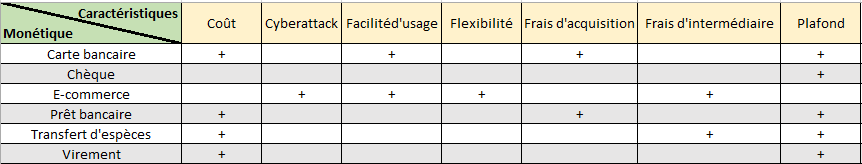
\includegraphics[width=1\textwidth]{tableau_recap}
\begin{center}
   \textbf{\underline{Récapitulatif du système actuel}} \\[1cm]
\end{center}


%%%%%%%%%%%%%% Blockchain %%%%%%%%%%%%%%
\newpage
\section{Blockchain dans les transactions}

\hspace{1cm} Nous vivons donc avec cette monétique qui nous permet d'effectuer des transactions bancaires, des transferts de fonds... Cependant ce système commence à semer les doutes dans l'esprit des utilisateurs. Il coûte de plus en cher et présente des failles de sécurité surtout avec la présence des cyberattacks sur le marché. Pour résoudre et faire face à ces problèmes, nous pouvons chercher d'autres méthodes pour assurer ces transactions. Et aucune autre technologie ne me vient en tête à part les blockchains. C'est vrai que c'est une nouvelle technologie, mais a déjà montré ses prouesses et semble avoir un avenir assuré. Je vais donc essayer de voir comment mettre en place les blockchains dans le monde monétaire et voir le rôle qu'elle peut jouer dans les différentes transactions.

%%%%%%%%%%%%%% Carte bancaire %%%%%%%%%%%%%%

    \subsection{Les cartes bancaires}

\hspace{1cm} Le système de la blockchain pourrait faire disparaître les contraintes liées aux cartes bancaires et nous offrir ainsi une meilleure gestion de nos transactions. Et quoi de plus beau que de pouvoir dépenser ses \textit{coins} dans la boulangerie en bas de chez soi? Pourtant c'est bien possible en mettant en place des cartes bancaires en crypto-monnaie. Cette carte est reliée à votre portefeuille, qui stocke "votre richesse". Et afin d'effectuer des transactions de manière décentralisée, le portefeuille doit en sorte être "multi-cryptos. C'est à dire donner accès à plusieurs devises virtuelles dans différentes chaînes de blocs , afin de ne pas imposer aux utilisateurs une unique monnaie. \\

\hspace{1cm} Et comment faire pour retirer en espèce? Obtient-on des euros ou des cryptomonnaies une fois devant le distributeur de banque ? Cela ne pose pas de problème majeur. La carte cryptomonnaie est avant tout une carte prépayée. Ce qui veut dire qu'elle peut être créditée qu'avec les devises actuelles comme EUR, USD ou GBP. Donc même si vous détenez des bitcoins cette monnaie sera convertit à la devise de votre choix au moment des retraits.\\

\hspace{1cm} Cette carte permettra aussi de dépenser ses cryptomonnaies chez le commerçant qui, à priori, n'a pas à y voir un quelconque inconvénient. En effet pour lui c'est comme une carte bancaire normale puisqu'il recevra son argent en euro. Tout simplement parce que la conversion crypto en euro est instantanée. Comment ça marche? Lorsque vous effectuez un paiement chez le commerçant, une vente instantanée du même montant en crypto est donc initiée. La carte est ensuite chargée du montant en euro, sans laisser de trace et sans que le commerçant même sans aperçoive.\\

\hspace{1cm} La carte sera transparente aussi pour tout ce qui est frais bancaire, donc pratiquement pas de frais du tout, même si une transaction en bitcoin coûte de plus en plus chère. Il faut afficher le continuellement les cours auxquelles les cryptomonnaies seront vendus en se basant sur sur plusieurs échanges afin de proposer le meilleur taux. Mais à vrai dire, un paiement sans frais n'existe pas, donc qui doit payer les frais? Sur ce point il n y aura pas de changement car ce sera le marchand qui paie comme dans les transactions bancaires actuelles.\\

\hspace{1cm} Cependant tout le monde n'est pas d'accord sur cette intégration. Prenons le cas de \textbf{Frédéric Dalibard}, responsable du digital de la banque de grande clientèle de Natixis, qui pense que remplacer un Visa par une blockchain est quasi impossible parce que, par exemple un bitcoin ne peut enregistrer seulement qu'une dizaine de transactions par seconde contrairement au Visa qui peut en faire \textbf{20 000}. Ce qui n'est pas faux car les paiements avec les cryptomonnaies ne sont pas instantanées. Avec Bitcoin, vous pouvez avoir un délai de \textbf{10 minutes} avant que le réseau n'inclut votre transaction dans un bloc. Et cette transaction est opérationnelle au moment où elle est validée.\\

\hspace{1cm} Nous avons aussi le processus de mise en place des outils nécessaires pour le marchand du quartier afin d'accepter les cryptomonnaies qui est assez simple mais un peu complexe . Un autre point bloquant, qu'il ne faut surtout pas oublier, est la sensibilisation des commerçants à accepter une monnaie dont le cours varie subitement d'une minute à l'autre.


%%%%%%%%%%%%%% E-commerce %%%%%%%%%%%%%%

    \subsection{Le e-commerce}
\textbf{E-commerce}

\hspace{1cm} Cette blockchain serait un grand atout pour ces e-commerçants. En effet la mise en place de cette technologie dans ce secteur supprimerait tous les intermédiaires entre vendeurs et acheteurs. Les e-commerçants pourront proposer des transactions se passant d'intermédiaires, donc ne plus verser de commissions aux plate-formes, aux organismes bancaires. Prenons un exemple sur Shopify et Paypal, qui sont des sociétés de paiement en ligne très populaires de grandes plate-formes de commerce. Elles prennent une commission de 1,5\% à 6\%. Cette redevance est transmise au client, ce qui rend les achats en ligne beaucoup plus chers.\\

\hspace{1cm} D'après \textbf{Thomas France}, co-fondateur de la Maison du Bitcoin à Paris, ce système pourrait faire économiser 3\% à 4\% des chiffres d'affaires des e-commerçants qui réalisent beaucoup d'opérations depuis de l'étranger. Effectivement, les transactions internationales sont souvent réalisées par l'intermédiaire des plate-formes tierces, les obligeant à débourser beaucoup de frais. Alors que les paiements en bitcoins ne génèrent aucun frais de transactions pour le vendeur. Ceci est un grand avantage pour les e-commerçants en quête de rentabilité absolue.\\

\hspace{1cm} L'inexistence des frais de transaction est assurée grâce au protocole de la blockchain dont le code source a la caractéristique d'être un open source. De même avec son fonctionnement sur le réseau de pair à pair, il n'y a pas d'autorité centrale ou intermédiaire. Ce qui fait que tout le monde peut contrôler ou posséder les bitcoins. Donc, quand une transaction est réalisée entre deux parties la monnaie ne passe par aucun intermédiaire et est échangée, comme presque un échange liquide. Ce qui fait que rien ne justifie des frais de transactions. De même une fois le paiement effectué, il devient irréversible, donc l'e-commerçant est aussi protégé contre des frais d'annulation de paiement de la part de l'acheteur. Par contre pour tout mécontentement de l'acheteur le cyber-marchand  peut toujours le rembourser contre le retour du produit acheté.\\

\hspace{1cm} \hspace{1cm} Nous avons aussi un élément clé qui peut vraiment révolutionner le e-commerce. On l'appelle les \textbf{ contrats intelligents} plus connus sous le nom de \textbf{smart contracts}, en anglais qui peuvent être une grande force pour le e-commerce. Ces contrats sont la véritable application derrière la technologie blockchain. Nous entrerons pas en détails sur là-dessus car il faudra tout un article entier pour vous en parler. Mais je peux vous dire que ces contrats sont en résumé des accords numériques entre des parties qui s'exécutent automatiquement quand les obligations ont été respectées et remplies. Si un acheteur valide son panier il envoie le prix fixé d'un produit en cryptomonnaie au contrat. Une fois le contrat reçu, le vendeur envoie la preuve de propriété  au smart contract et en même temps il va lier ce contrat au transporteur du produit vendu. Dès que toutes les obligations sont remplies, le contrat enverra automatiquement l'argent au porte-monnaie du vendeur qui pourra les récupérer et utiliser à tout moment. Ainsi ces contrats permettent de faire des transactions directes entre les acheteurs et les vendeurs sans frais et avec une simplicité remarquable.\\
    
\hspace{1cm}Par conséquent mettre en place le paiement par les crypto-monnaies n'est pas sans présenter certains risques pour les professionnels de la vente en ligne. En effet le système est très volatile. La monnaie est soumise à la loi de l'offre et de la demande, ce qui fait que le prix augmente quand la demande est forte et diminue lorsque la demande est faible. Donc son cours est très instable et évolue de manière imprévisible, en témoignent les fortes fluctuations de son prix ces derniers mois, à des périodes très rapprochées. Le montant perçu lors d'une vente peut varier entre le moment de l'achat et celui de la réception du paiement. Voir \textbf{annexe 1} \\

%%%%%%%%%%%%%% Les transactions sur papier %%%%%%%%%%%%%%

    \subsection{Les transactions par documents}
\hspace{1cm} Et si nous nous tournions vers les blockchains pour voir les propositions que peut nous faire cette technologie à propos des transactions par papier? En fait l'idée serait de mettre des codes QR unique et spécifique à chaque chèque. Ce code sera enregistrer en amont sur la blockchain, ce qui permettra de vérifier et l'authenticité du chèque et de le valider. \\

\hspace{1cm} Nous pouvons mettre ici aussi en avant les smart contracts qui sont très puissants. Ils ne s'appliquent pas seulement dans le e-commerce. La même logique avec le même procédé décrit dans les e-commerces peut également s'appliquer sur les transactions par billet à ordre, sur les lettres de change ainsi que sur les traites.\\

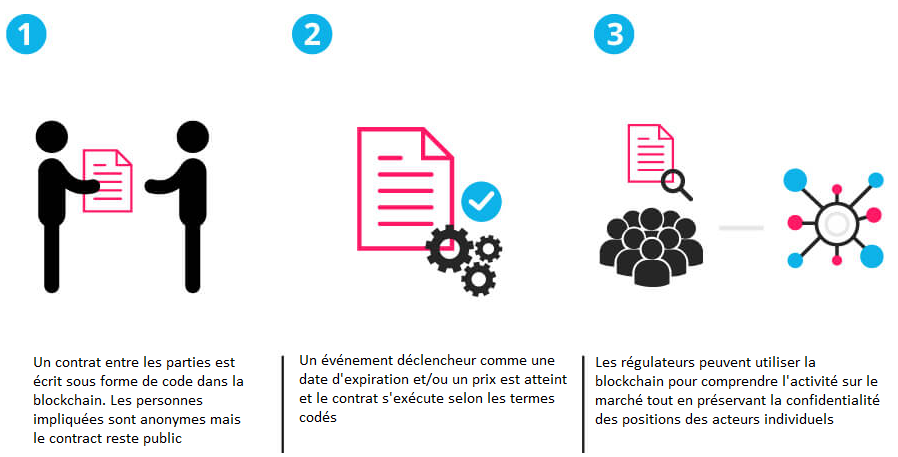
\includegraphics[width=1\textwidth]{contract_smart}
\begin{center}
   \textbf{\underline{Processus d'un smart contract}} \\[1cm]
\end{center}

%%%%%%%%%%%%%% Transfert d'argent %%%%%%%%%%%%%%

    \subsection{Virements}
    
\hspace{1cm} Ces virements qui prennent des jours pour arriver à destinations avec des coûts chers peuvent prendre fin. 

REQ, permet à l’utilisateur d’effectuer des transactions de manière transparente, sécurisée et à moindre coût, via la blockchain. Leur livre blanc estime actuellement les frais de 0,05 à 0,5pcent par transaction, les frais diminuent à mesure que le volume du réseau augmente puisqu’une partie des frais perçus sont brûlés et partiellement utilisés pour financer le réseau.\\

La blockchain pourrait alors constituer une solution infiniment moins coûteuse (seuls quelques centimes sont prélevés sur chaque transaction) et plus rapide (entre 10 mn à 1h, contre parfois plusieurs jours pour les transferts à l’étranger)

%%%%%%%%%%%%%% Western Union et moneygram %%%%%%%%%%%%%%

    \subsection{Western Union \& MoneyGram}

%%%%%%%%%%%%%% Prêt bancaire %%%%%%%%%%%%%%

    \subsection{Faire un prêt! }
ETHLend est une application décentralisée sur la blockchain de l’Ethereum permettant d’effectuer des prêts entre particuliers de façon sécurisée et transparente.
C’est un moyen efficace pour les emprunteurs d’accéder à des financements à l’échelle mondiale et pour les prêteurs de financer des demandes de prêts à travers le monde.

ETHLEND DÉCENTRALISE LA FINANCE


râce à la blockchain de l’Ethereum, ETHLend décentralise la finance pour créer un marché mondial du crédit. Ainsi, un emprunteur au Brésil n’est pas limité aux prêteurs locaux et aux banques brésiliennes, il peut en effet accéder à des financements venant d’Asie, d’Amérique du Nord ou d’ailleurs.

Cela signifie pour les prêteurs davantage de possibilités d’investissement. ETHLend permet donc l’internationalisation du marché du crédit ainsi qu’un accès plus rapide à celui ci par rapport à l’utilisation du système bancaire. Les transactions sont effectuées en quelques secondes ou minutes comparés aux jours d’attente que l’on rencontre dans le système bancaire traditionnel.
Par ailleurs, en offrant plus de liquidités au niveau local ETHLend favorise la compétition sur les taux d’intérêts et grâce à l’utilisation de cryptomonnaies, il n’est pas nécessaire d’avoir un compte en banque pour obtenir un prêt.

%%%%%%%%%%%%%% Conclusion du chapitre %%%%%%%%%%%%%%
\hspace{1cm} Les cryptomonnaies ont donc la capacité de fournir des solutions aussi bien pour le e-commerçant que pour l'acheteur en supprimant  le besoin d'un tiers. Ces monnaies peuvent également être meilleures que les services de portefeuille numérique de nos jours car la blockchain nous permet: 
    \begin{itemize}
        \item De faire des transactions instantanées avec des frais peu élevés
        \item A n’importe qui d'en bénéficier
        \item De ne pas fournir fournir ses informations personnelles et financièrement sensibles aux tiers.
    \end{itemize}

-------------------


\newpage		
\section{Conclusion}

\hspace{1cm} 

--------------
Un défaut majeur dans la façon dont nous stockons actuellement les données est qu’elles sont stockées dans un endroit central et contrôlées par une partie centrale. Oui, les cybercriminels peuvent pirater des individus, mais ils ne voleront que les informations de l’individu qu’ils piratent. Il est pratiquement impossible de pirater une blockchain entier.\\
----------------

\hspace{1cm} La blockchain est devenue un sujet incontournable cette année.Grâce au réseau et à la cryptographie, elle a un système sécurisé qui pousse les particuliers et les entreprises à l'utiliser sans besoin de faire appel à des intermédiaires. Les seuls frais possibles à payer sont la maintenance et la sécurisation du réseau. Pour un acheteur et un vendeur, techniquement il y a aucun frais à dépenser puisque les plates-formes du e-commerces seront des applications blockchain. Ainsi les utilisateurs détermineront le développement et le fonctionnement de la plate-forme car les blockchains sont décentralisées, pas de partie centrale ou de société qui décide ou définit les règles.\\

\hspace{1cm} 

-----------------------\\



Le grand public est encore peu familiarisé avec cette monnaie alternative, dont le fonctionnement tranche résolument avec les devises monétaires habituelles. Sa démocratisation demeure encore hypothétique et il est difficile d’évaluer l’importance qu’elle pourrait prendre dans les années à venir.

Malgré le coût potentiel d'implémentation, la blockchain dispose tout de même d'avantages incontestables en termes de rapidité et de sécurité.

Aujourd'hui, les systèmes de paiement fonctionnent plutôt bien, renchérit de son côté Grégory Chenue, du Crédit Agricole. Tout casser pour remplacer par des systèmes blockchain prendrait beaucoup de temps car on ne part pas de zéro, les infrastructures de réseau sont très complexes."


 Le caractère décentralisé de cette nouvelle technologie, couplé avec sa sécurité et sa transparence, fait des prouesses aujourd’hui.
 
 Depuis, de nombreuses institutions bancaires s’y intéressent et réalisent des transactions mais le débat reste entier : doit-on réguler ces monnaies virtuelles ? Comment contrôler la fluctuation de celles-ci ? \\

\newpage
\section{Webographie}

\newpage
\section{Annexes}

\textbf{Annexe 1}\\
\begin{center}
    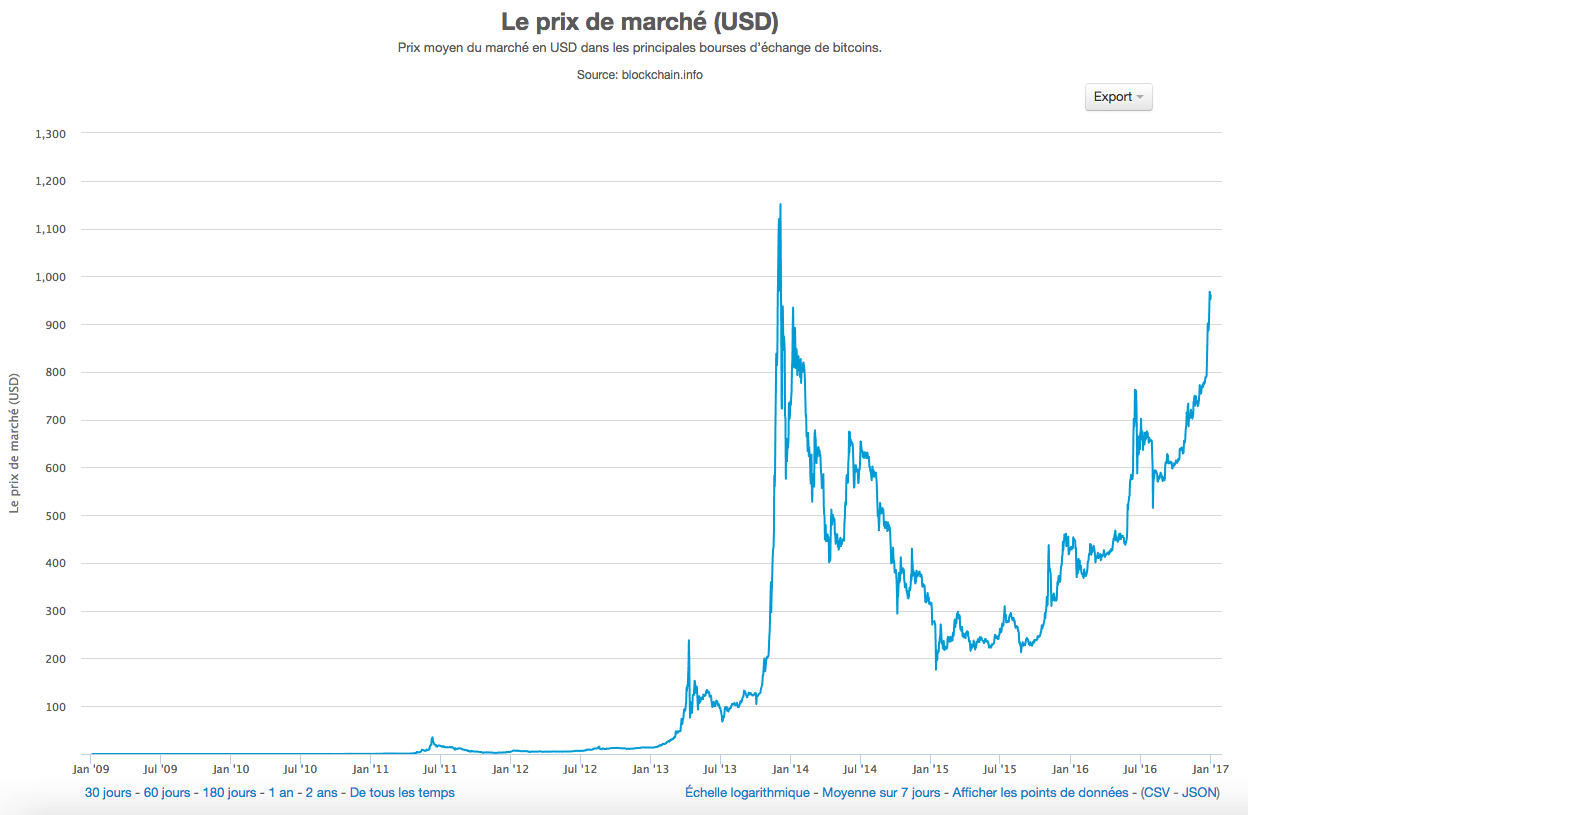
\includegraphics[width=1.3\textwidth]{courbeBTC}
\end{center}

\end{document}